\documentclass{beamer}

\title{Isabelle/HOL on Fork Prevention\\ in the Coming Ethereum Protocol}
\author{Yoichi Hirai\\ {\small Ethereum Foundation}}
\date{Berlin, 30 Aug. 2017}

\begin{document}

\begin{frame}
\titlepage
\end{frame}

\begin{frame}{What is Ethereum}

Ethereum is one-instance of a virtual machine
\begin{itemize}
\item as powerful as a 20-year-old smart phone
\item replicated globally
\item with no central parties
\item running for 2 years by now
\end{itemize}

\vfill

How does Ethereum synchronize execution traces? \\
Asynchronous communication cannot establish new common knowledge.
\end{frame}

\begin{frame}{Blockchain}
is just a data strucuture.  It is a tree, not a chain.

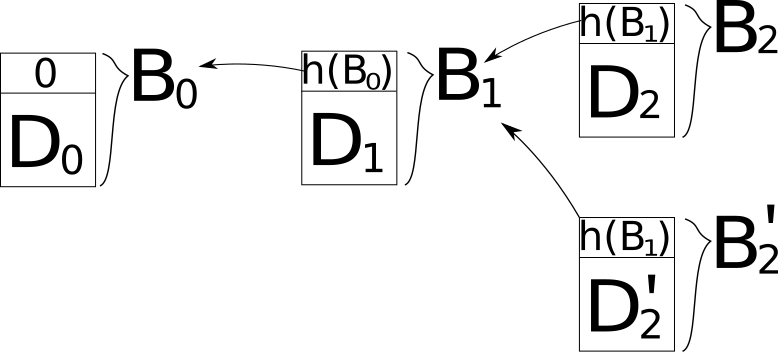
\includegraphics[width=\textwidth]{blockchains.png}

A small number $h(B_n)$ identifies a sequence $B_0, \ldots B_n$ and \\
moreover, in Ethereum, the execution trace of a virtual machine.

\end{frame}


\begin{frame}{Proof of Work}

\begin{itemize}
\item a block's content $D$ needs to contain a nicely chosen nonce\\ so that the hash $h(D)$ of the block is small enough
\item when you find such a nonce, the protocol gives reward in your account (in the state after the block)
\item account?
\end{itemize}

Finding a good nonce is called \structure{mining}.

I belive nobody has found a better way than brute-force.
\end{frame}

\begin{frame}{Proof of Work}

\structure{If you succeed creating a block}
\begin{enumerate}
\item the block reward is only spendable in chains that include your block
\item you should send around the block, maybe
\end{enumerate}

\structure{If you see a block being sent around}
\begin{enumerate}
\item if that's the best block you've seen, you should try to mine on the block \\
      (assumption: absense of complicated motives, other nodes' straightforward behavior)
\item you should broadcast the block you are mining on, maybe
\end{enumerate}

\structure{Does it work?}  Yes, see Bitcoin.

\structure{Why?}  I don't know, honestly.
\end{frame}

\begin{frame}{Evaluating Proof of Work}

No good properties distributed-computation-wise.

(A good leader-election protocol can tolerate less than 1/3 Byzantine nodes.)

\structure{One Byzantine node can}
\begin{itemize}
\item be lucky enough to guess the secret keys of all public keys it sees.
\end{itemize}

\structure{One (economically) irrational node can}
\begin{itemize}
\item buy lots of machines to mine quicker than anybody, rewriting the history from any point.
\end{itemize}

\structure{Why would anybody choose this?} \underline{number of nodes} is not reliable.

Instead, Proof-of-Work uses electricity consumption (or luck).

Instead, Proof-of-Stake uses in-protocol deposit.

These designs require numbers that carry values.

\end{frame}


\begin{frame}{Proof-of-Stake}

Replacing GPU and electricity with deposits of in-protocol tokens.

The deposits are made in some common anscestors of all considered blocks.

Provably dishonest behavior is punished, the deposits are gone on all chains.

(TODO: see ``nothing at stake problem'') again

What about cases hard to determine who violated the rules?

Two parties blaming each other is already bad enough.
\end{frame}


\begin{frame}{Some definitions}
When I was in Paris I received the following definitions.

(paste the definitions)
\end{frame}

\begin{frame}{Alloy modelling}
Being unsure what it meant, I turned to Alloy.
\end{frame}


\begin{frame}{Isabelle/HOL}

\end{frame}


\begin{frame}{Other formal verification projects}
\end{frame}

\end{document}
